\section{Converter Simulation Results}
% The simulation results presented should validate that the design meets the specification.

% Include diagrams and figures to support your presentation of results. 
% There should be a diagrams/figures that clearly show how the design specification have been met. 
% Ensure that all diagrams are legible, have axes with units and have captions which describe the diagram.

%In addition to presenting the simulation results include an answer to the following questions. In your report clearly indicate the question and the answer.

\begin{figure}
	\centering
	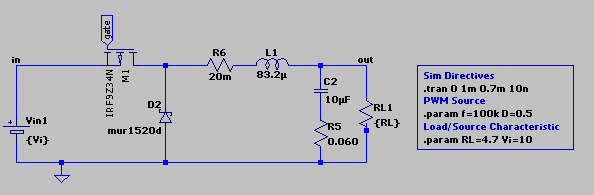
\includegraphics[width=\linewidth]{img/ConverterCircuit}
	\caption{Converter circuit. \texttt{gate} is the PWM source.}
	\label{fig:convertercircuit}
\end{figure}
\begin{figure}
	\centering
	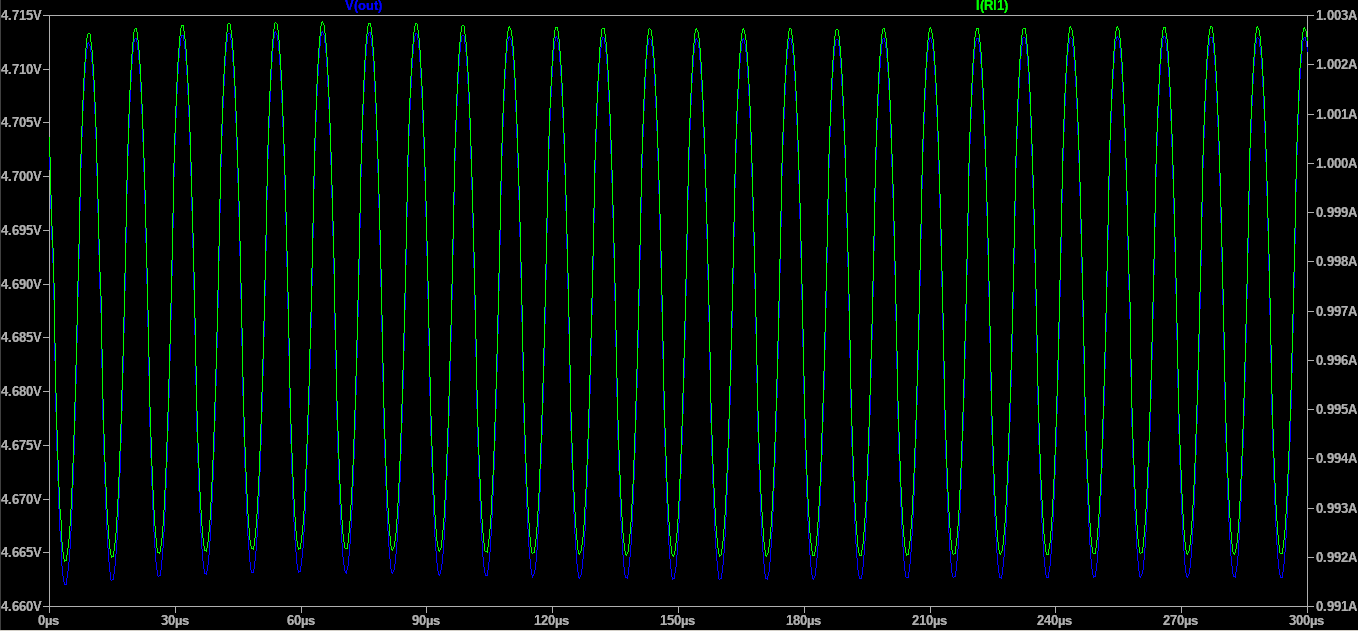
\includegraphics[width=\linewidth]{img/ConverterSimulationResults}
	\caption{Converter output voltage and current}
	\label{fig:convertersimulationresults}
\end{figure}

\Cref{fig:convertercircuit} gives the final converter circuit and \cref{fig:convertersimulationresults} the output voltage and current. The former has a dc value of \SI{4.6875}{\volt} with a ripple of \SI{50}{\milli\volt} and the latter a dc value of \SI{997.34}{\milli\ampere} with a ripple of \SI{11}{\milli\ampere}.

\subsection{Questions}
\subsubsection{What is the minimum gate voltage that can be used to drive the high side switch?}
% Explain your answer.
The high side switch is a PMOS. For it not to be in cut-off, the gate voltage must be less than a threshold below the source voltage. Since the source voltage is at the input voltage, this means that the gate voltage must always be at least a threshold below the input voltage. The minimum gate voltage for which conduction is guaranteed is therefore $V_{in,max}+V_t=12-2=\SI{10}{\volt}$ ($V_t=\SI{2}{\volt}$ from datasheet).
\subsubsection{What would be the implications for the required high side switch gate voltages of if an NMOS switch is used instead of an PMOS?}
Since the gate voltage for the PMOS is lower than the input voltage used for the converter, a voltage divider can be used to drive it from the input voltage. An NMOS would require a gate voltage higher than the input and corresponding circuitry to increase the voltage.
\subsubsection{In terms of how well the design meets the specifications, do the design calculations and results from the simulation agree?}
Both the voltage and current ripples are within specifications.
\subsubsection{What is the efficiency of the converter determined from the LTSpice simulation?}
% Note you can calculate power loss for components directly in LTSpice.
The power input to the converter is \SI{7.4215}{\watt} from the input voltage and \SI{7.3221}{\milli\watt} from the pwm source. \SI{4.5469}{\watt} is dissipated in the load. This gives an efficiency of 61\%.  
\subsubsection{Does this efficiency agree with the calculated efficiency? If not why not? What is different between the calculations and the simulation?}
The measured efficiency is so similar to the calculated efficiency of 65\% that it leads me to suspect some error in the calculations.
The total simulated inductor loss was \SI{39.649}{\milli\watt} rather than the calculated \SI{1.56}{\watt}. This could indicate an error in calculations.
\subsubsection{Under what conditions does the converter enter discontinuous conduction mode?}
When the duty cycle is too high, the switching frequency is too low, or the output current is too low.


